\section{Virtual Reality}
With the launch and success of modern technologies like Oculus Rift, HTC Vive or Playstation VR (Figure \ref{fig:CONTROLLERS}), today’s virtual reality (VR) is mostly associated with a head-mounted device that provides this experience for the wearer. Virtual reality headsets combine a stereoscopic head-mounted display (HMD), stereophonic sound, and sensors like gyroscopes or accelerometers for head motion tracking. The main goal of these devices is to fool user’s senses, make him feel present and immersed in virtual reality. A person using such equipment is able to move and look around artificial world. Usually users can also interact with its features in some way, using specially designed controllers. Today VR headsets are mostly used for gaming, simulations, education, and other entertainment purposes.

\begin{figure}[th]
\centering
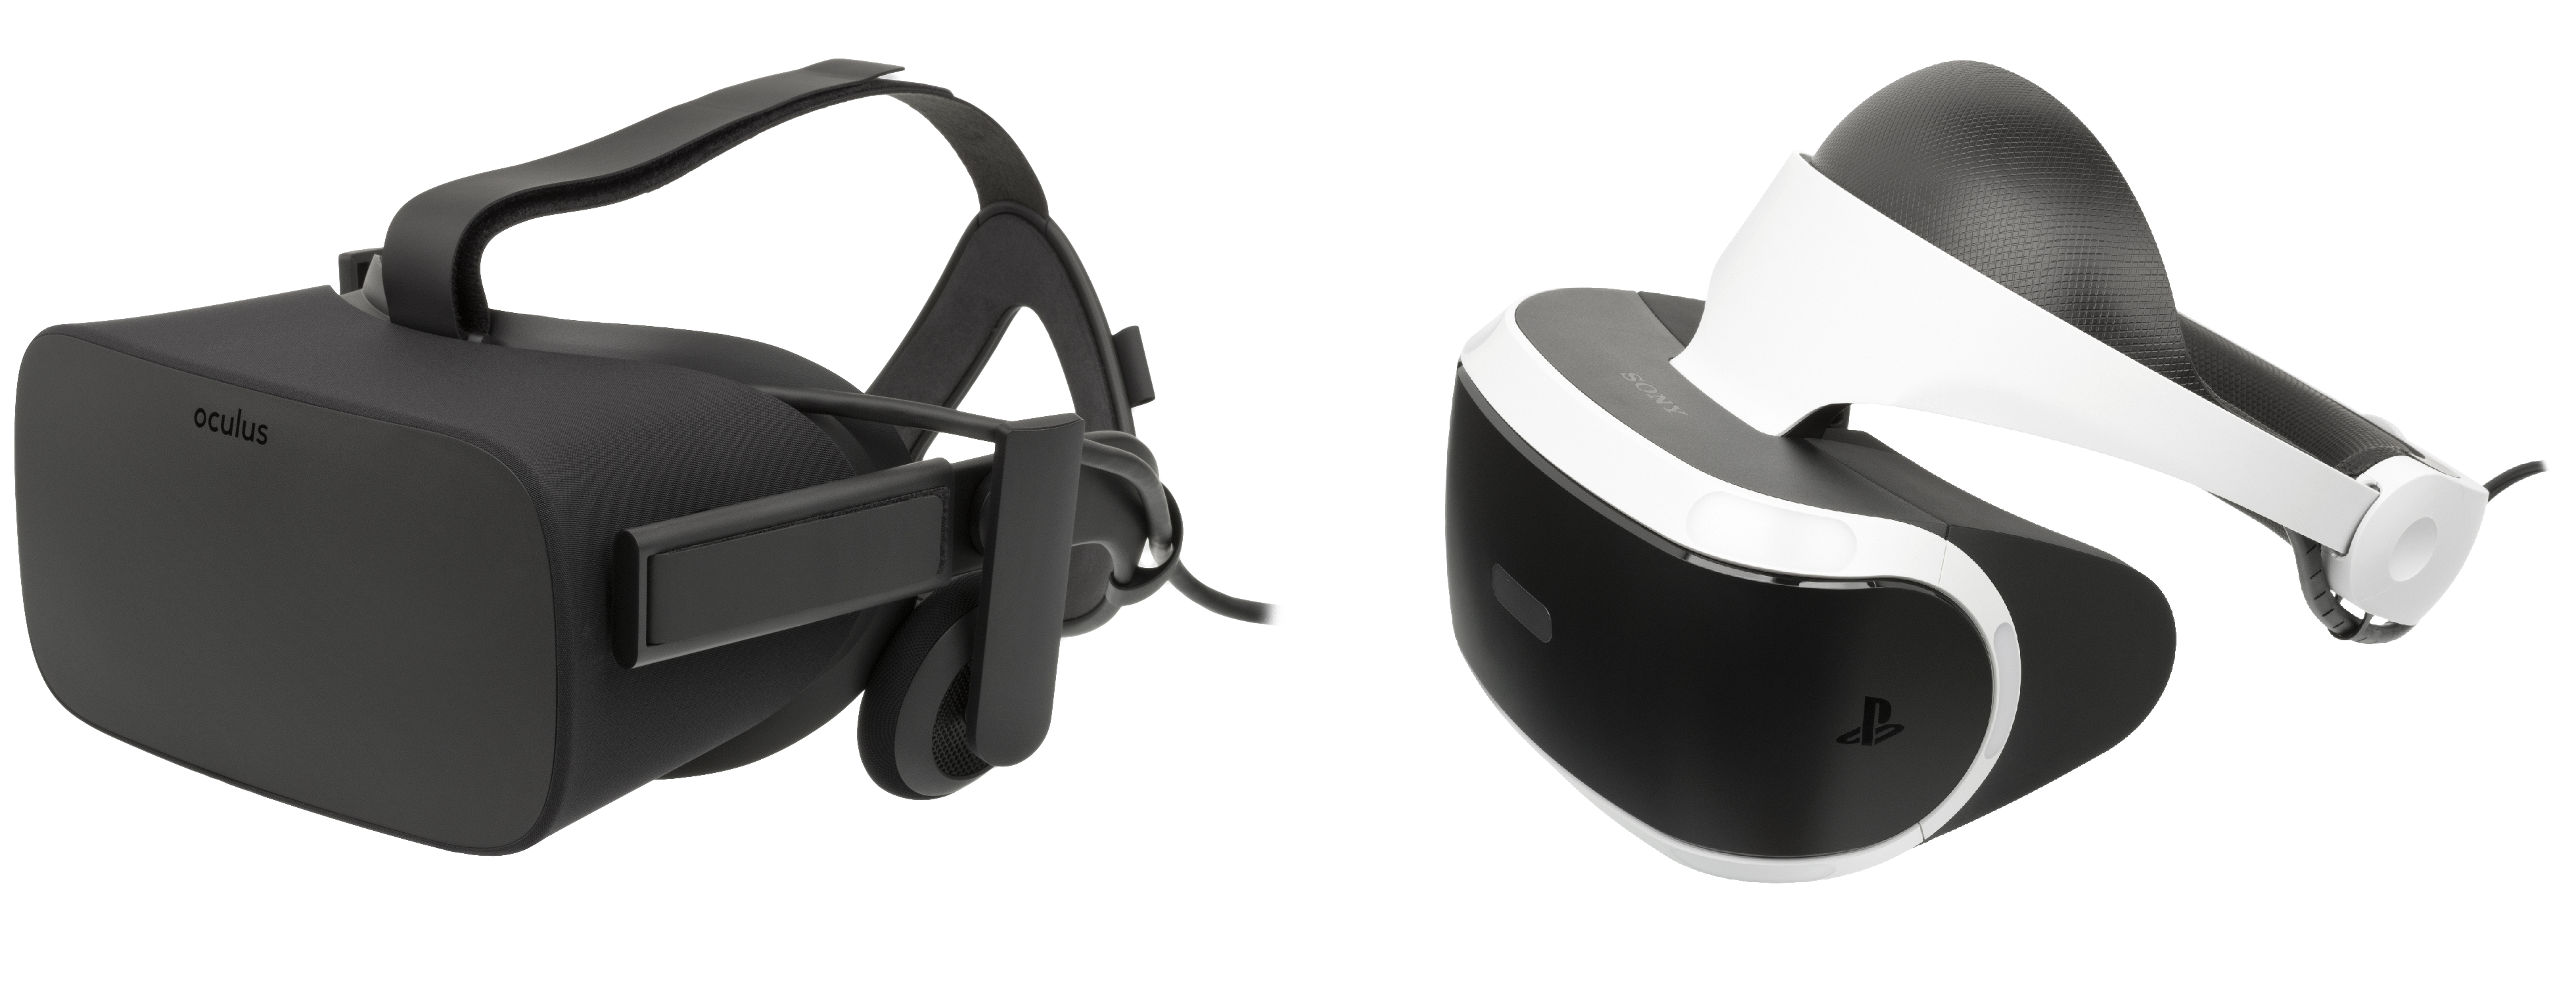
\includegraphics[width=1\textwidth]{img/headsets.png}
\caption{Modern popular VR headsets: Oculus Rift and Playstation VR (source: \cite{OCULUS_HEADSET}\cite{PSVR_HEADSET})}
\label{fig:CONTROLLERS}
\end{figure}

The concept of virtual reality is evolving and changing quickly. The technologies we use now will probably become obsolete in next 5 years. To describe what virtual Reality really means, we must be broad enough to enclose what it meant in the past, what it is today, and what it can become in the future. S. M. LaValle in his book \cite{VR_BOOK} tries this approach to define VR in general way. The four key concepts which appear in his VR definition are:

\begin{itemize}
\item \textit{Targeted behavior}: The experience from the real world we try to replicate. It could be anything from walking, dancing, swimming, shooting arrows, etc.
\item \textit{Organism}: Any life form can be the user of VR. In the past it was tested even on animals like cockroaches, fishes, monkeys and rodents.
\item \textit{Artificial sensory stimulation}: With the use of available equipment and technology, organism’s senses are tricked to make him feel present in artificial reality.
\item \textit{Awareness}: While being immersed in VR, the user should be oblivious to any interference. Feeling presence in this altered or another world is accepted as natural.
\end{itemize}

Virtual reality has a long history and can be traced back even to 1962, when Morton Heilig built a machine called Sensorama. It could provide body tilting, supply stereo sound, display stereoscopic 3-D images, and was able to trigger tracks of aromas and wind during the film \cite{SENSORAMA}. Later in 1968, Ivan Sutherland invented what is regarded as the first head-mounted display device: The Sword of Damocles. The system provided basic user interface and realism, the graphics of created VR were simple wire-frame model rooms \cite{DAMOCLES}. The device was so heavy that it had to be attached to the ceiling with a mechanical arm (Figure \ref{fig:FIRST_VR}). In the next years VR devices were mainly used for flight simulation, military training, medical purposes and automobile design. Advancements in technology and the launch of an affordable high-quality VR headsets, made virtual reality more accessible for video game players. Today we are witnessing an exciting rebirth of interest in VR, not only in entertainment industry but also in academic research.

\begin{figure}[th]
\centering
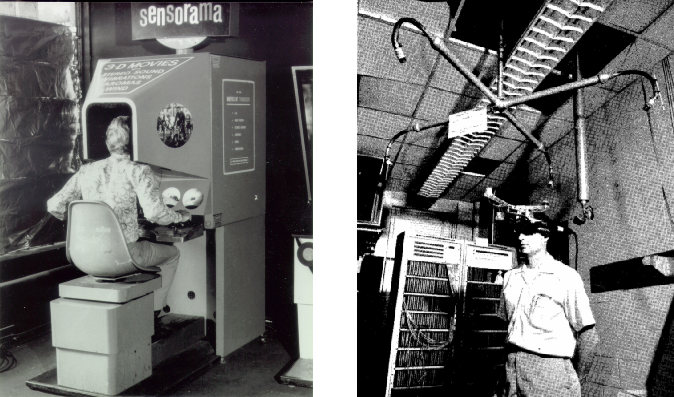
\includegraphics[width=0.9\textwidth]{img/first_vr.png}
\caption{The Sensorama and The Sword of Damocles, first attempts at creating virtual reality (source: \cite{SENSORAMA_IMAGE}\cite{DAMOCLES})}
\label{fig:FIRST_VR}
\end{figure}

\section{VR input methods}

As more companies enter the VR headset market, we can see the rapid technological advancement in input devices. Authors of the article \textit{State of the Art of Virtual Reality Technology} \cite{VR_TECHNOLOGY} identified three different categories for devices handling input in VR: controllers, navigation devices and tracking technologies. Most of the controllers for VR headsets are hand worn and provide 6DoF (Six Degrees of Freedom) tracking information. They are usually equipped with buttons for discrete input, and top-mounted touchpads or joysticks for analog input (Figure \ref{fig:CONTROLLERS_IMAGE}).

\begin{figure}[th]
\centering
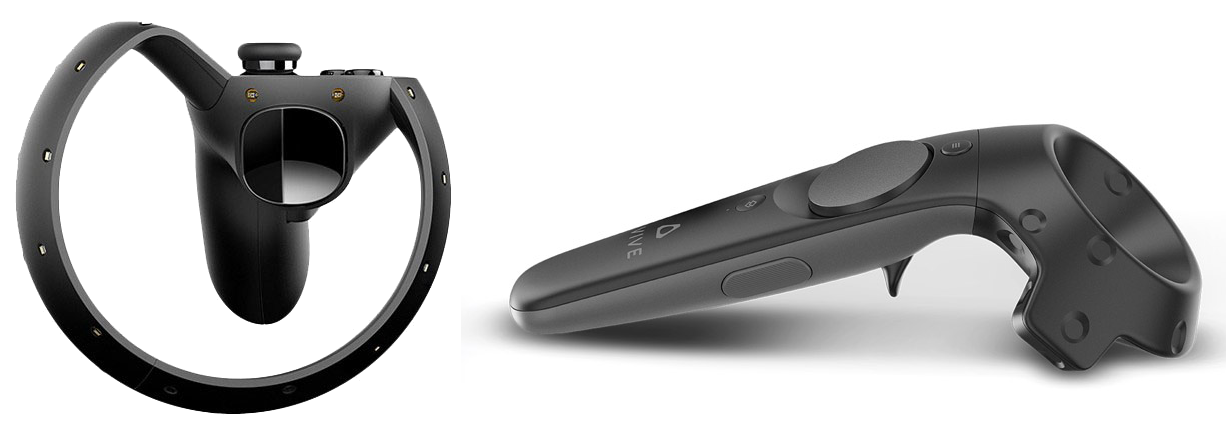
\includegraphics[width=1\textwidth]{img/modern_controllers.png}
\caption{Modern VR controllers: The Oculus Touch and HTC Vive Controller (source:  \cite{VR_TECHNOLOGY}\cite{VIVE_IMAGE})}
\label{fig:CONTROLLERS_IMAGE}
\end{figure}

The illusion of traversing an endless space can be achieved with the help of navigation devices which are an input source for moving in the virtual environment. Most devices in this category act similar to traditional treadmills allowing movement in one direction. Some of them allow motion on a two-dimensional plane or function like the slidemills. For example, Virtuix Omni (Figure \ref{fig:VIRTUX_IMAGE}) is a concave platform with a low-friction surface which allows locomotive motion in any direction. There are also attempts at creating devices less expensive and more affordable to general public. Google is currently working on motorized shoes that allow an endless movement in a limited space \cite{VR_SHOES}. Other researchers try to use devices which were not specially designed for virtual reality. For instance, A. Aguirre in his master thesis \cite{JOYSTICK} describes the process of navigation in VR through leaning on Wii Balance Board.

\begin{figure}[th]
\centering
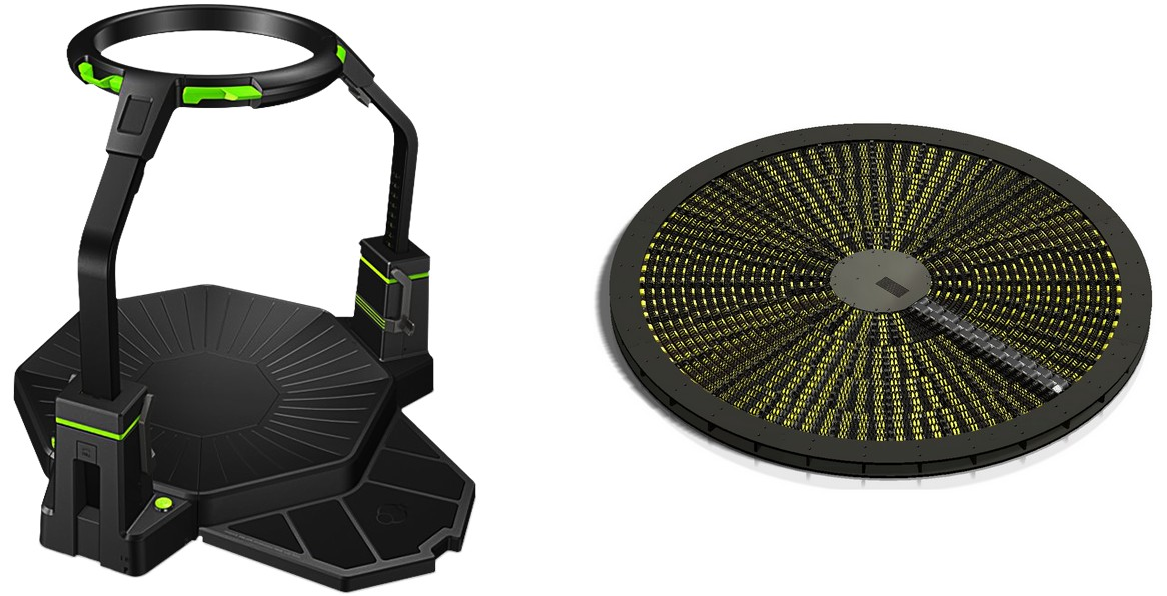
\includegraphics[width=0.9\textwidth]{img/vr_threadmills.png}
\caption{Omnidirectional treadmills: Virtuix Omni and WalkMouse (source:  \cite{VR_TECHNOLOGY})}
\label{fig:VIRTUX_IMAGE}
\end{figure}

There are currently two approaches for motion tracking technologies. First is full body tracking which focuses on posture and upper body of the users. Second is gesture tracking which is usually achieved optically or with devices worn on hands. Full body tracking is commonly implemented using magnetic tracking or Inertial Measurement Units (IMUs), providing six degrees of freedom by placing orthogonally to each other accelerometers, gyroscopes and magnetometers. Valve came up with different approach, their Lighthouse positional tracking system involves two base stations that scan the area around room with lasers \cite{VIVE_STATION}. There are also various sensor technologies designed to be worn like a glove which are used to capture gestures such as bending of fingers. One of these data gloves called Gloveone, enables users to feel and touch any virtual object that they can see in VR headsets \cite{GLOVEONE}. There are 10 actuators distributed along the fingertips and palm of the glove, which vibrate independently at different intensities and frequencies, reproducing touch sensations.

\section{Virtual reality sickness}

While VR is a promising technology, which quickly gains on popularity, it still has a great challenge and safety issue to overcome. Virtual reality sickness (also called cybersickness) is a group of unpleasant symptoms which can occur during an exposure to virtual environment. These symptoms can last from few minutes to even days and most often include headache, disorientation, sweating, eye strain, fullness of stomach, pallor, vomiting, nausea, dryness of mouth, vertigo, or ataxia \cite{VRSYMPTOMSTIME}. Although similar to motion sickness, VR sickness is different in that it can occur with visual stimulation alone. Motion sickness is mainly induced with vestibular stimulation, while vision can be a contributing cause. It is also sufficiently different from simulator sickness which tends to occur as a result of oculomotor disturbances, with disorientation being the main symptom in VR sickness \cite{VRANDSIMULATORSICKNESS}. Beyond the sickness itself, these undesirable symptoms may have other consequences. VR sickness could reduce the efficiency of VR training and rehabilitation tools, or it could even discourage users from trying virtual reality ever again. Currently, there are many speculations as to why VR sickness occurs. J. J. LaViola in his article about cybersickness \cite{VRSYMPTOMS} describes three following main theories: 

\begin{itemize}
\item \textit{The sensory conflict theory}: The most commonly accepted theory which is based on the assumption that inconsistency between the vestibular and visual sense cause a perceptual conflict within the body. These sensory conflicts may appear when the sensory input is not the stimulus that the user expected based on his prior experience. Taking this into consideration, the symptoms of VR sickness could be reduced if the sensory information causing self-motion are in agreement with each other.
\item \textit{The poison theory}: The theory tries to explain VR sickness from an evolutionary standpoint. It is based on the premise that the consumption of poison leads to physiological problems which affects the coordination of sensory information. This serves as an early warning system that causes nausea and vomiting which may increase the chances of survival. The conflicting stimulation found in VR can cause the misreading of sensory inputs and make the body think that it has been poisoned.
\item \textit{The postural instability theory}: This theory focuses on the concept that the main objective of human body is to sustain postural stability at all time. If the control can't be maintained, the motion sickness symptoms appear. In many virtual environments, there are some optically specified movements which are abnormal for inexperienced users. As a result, their postural control strategies may fail.
\end{itemize}

There are also other contributing factors to VR sickness, not necessarily related to any of these three theories. Various technical aspects can have great impact on sickness symptoms, such as mismatched motion, low refresh rate, or not achieving the target frame rate. Head position tracking is a vital element of any virtual environment, however, current tracking systems are not completely accurate. They can report information with error which leads to uncontrollable movement and dizziness of the user. Studies have shown that increasing field of view (FOV) tends to increase VR sickness. Implementing methods to dynamically restrict FOV can help combat this effect \cite{DYNAMICFOD}. Several other techniques are used to reduce sickness symptoms. For example, introducing static visual background (Figure \ref{fig:STATIC_BACKGROUND}) allows users to register a verification of their senses, while simultaneously observing the full locomotion of virtual environment. It has also been noted that some individuals are more susceptible than others to VR sickness \cite{VRINDIVIDUALS}. Age, health, postural stability, gender, experience with the system, and many other factors can contribute to the severity of the symptoms.


\begin{figure}[th]
\centering
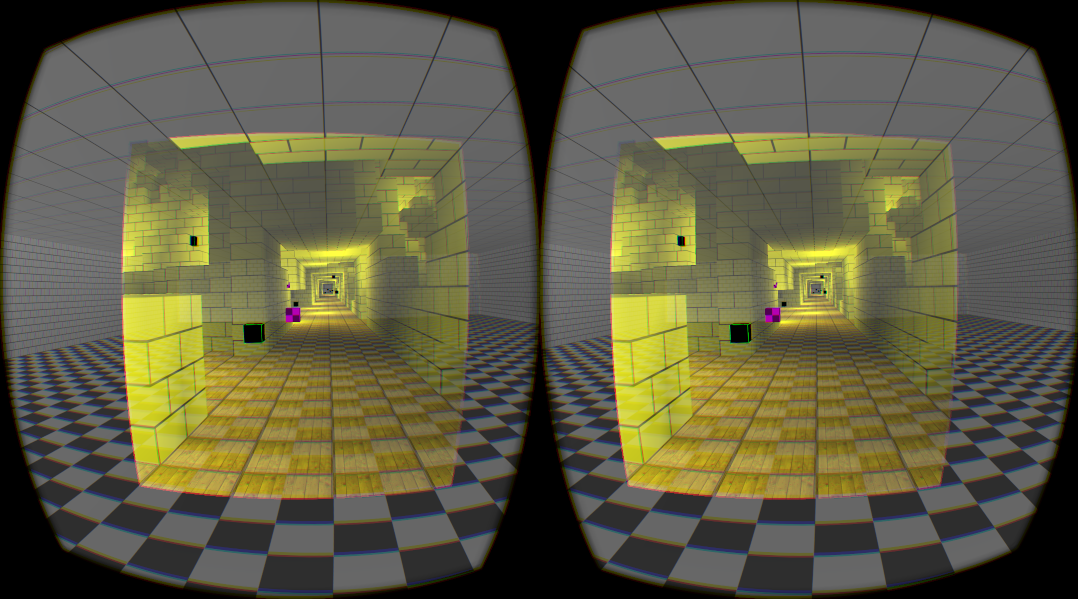
\includegraphics[width=0.9\textwidth]{img/static_background.png}
\caption{Static visual background, a technqiue used to reduce VR sickness symptoms (source:  \cite{STATICBACKGROUND})}
\label{fig:STATIC_BACKGROUND}
\end{figure}

\section{Locomotion in VR}




